% !TeX root = ../../../main.tex
\subsubsection{Diagnosis Distribution Analysis}
\label{ch05:diagnosis-distribution-analysis}

To characterize diagnostic coverage, we prompted the LLM to act as an expert physician and list patient-specific diagnoses for each case report. 
The prompt asked the model to extract final diagnostic labels (e.g., ``acne'', ``DRESS syndrome'') rather than isolated clinical findings (e.g., ``rash'', ``leukocytosis''), to place the primary diagnosis first, and to output one diagnosis per line without explanatory text (full prompt in Supplementary Material, Section~\ref{ch05:apd:diagnosis-prompt}).

Free-text diagnoses were then standardized to the Unified Medical Language System (UMLS) using the ScispaCy entity linker (\texttt{en\_core\_sci\_lg}) with the UMLS knowledge base. 
\ChFiveRebuttal{
Each complete extracted diagnosis string was supplied directly to the UMLS candidate generator, with candidate selection designed to avoid fragmentation and improve canonical concept assignment (Supplementary Material, Section~\ref{ch05:apd:umls-mapping}).
}

Figure~\ref{ch05:fig:top_diagnoses} shows the 20 most frequent UMLS-normalized diagnoses in PMOA-TTS.
These are dominated by common cardiometabolic and renal conditions, including hypertensive disease, diabetes mellitus and its subtypes, coronary artery disease, dyslipidemia, and chronic kidney disease.
\ChFiveRebuttal{
Figure~\ref{ch05:fig:diagnoses} characterizes diagnoses represented within PMOA-TTS; it is not an evaluation of diagnostic recognition. Common diagnoses may appear as comorbidities in reports whose primary focus is a rare or atypical presentation.
}

We further examined co-occurrence structure using a clustered heatmap of diagnosis pairs (Figure~\ref{ch05:fig:diagnosis_cooccurrence}).
The heatmap reveals coherent groupings among related conditions, most notably across diabetes variants, as well as broader co-occurrence patterns among cardiovascular, metabolic, and renal diagnoses.
These patterns are consistent with well-established comorbidity relationships (e.g., hypertension with diabetes, or atrial fibrillation with coronary artery disease) and illustrate how the corpus captures clinically meaningful disease constellations.

\ChFiveRebuttal{
To characterize rare-disease representation more directly, we matched UMLS CUIs associated with extracted diagnoses against disorder-level entities in the Orphanet rare-disease nomenclature \citep{lucano2026orphanet} using exact, validated UMLS mappings. After excluding groups and subtypes of disorders and entities designated as inactive, historical, deprecated, obsolete, or non-rare, the reference contained 5,942 Orphanet disorders. Overall, 41{,}775 of 124{,}349 reports (33.6\%) contained at least one extracted diagnosis mapped to an eligible Orphanet disorder, spanning 2,426 distinct ORPHAcodes. Across all extracted diagnoses, 50,299 of 474,075 mappings (10.6\%) matched the Orphanet reference. These statistics characterize rare-disease representation within PMOA-TTS rather than population prevalence.
}


% !TeX root = ../../../main.tex
\begin{figure}[htbp]
\begin{ChFiveFloatBody}

    \centering
    \subfloat[{Most frequent diagnoses.}]{\begin{minipage}[t]{0.39\textwidth}
        \centering
        \raisebox{40pt}{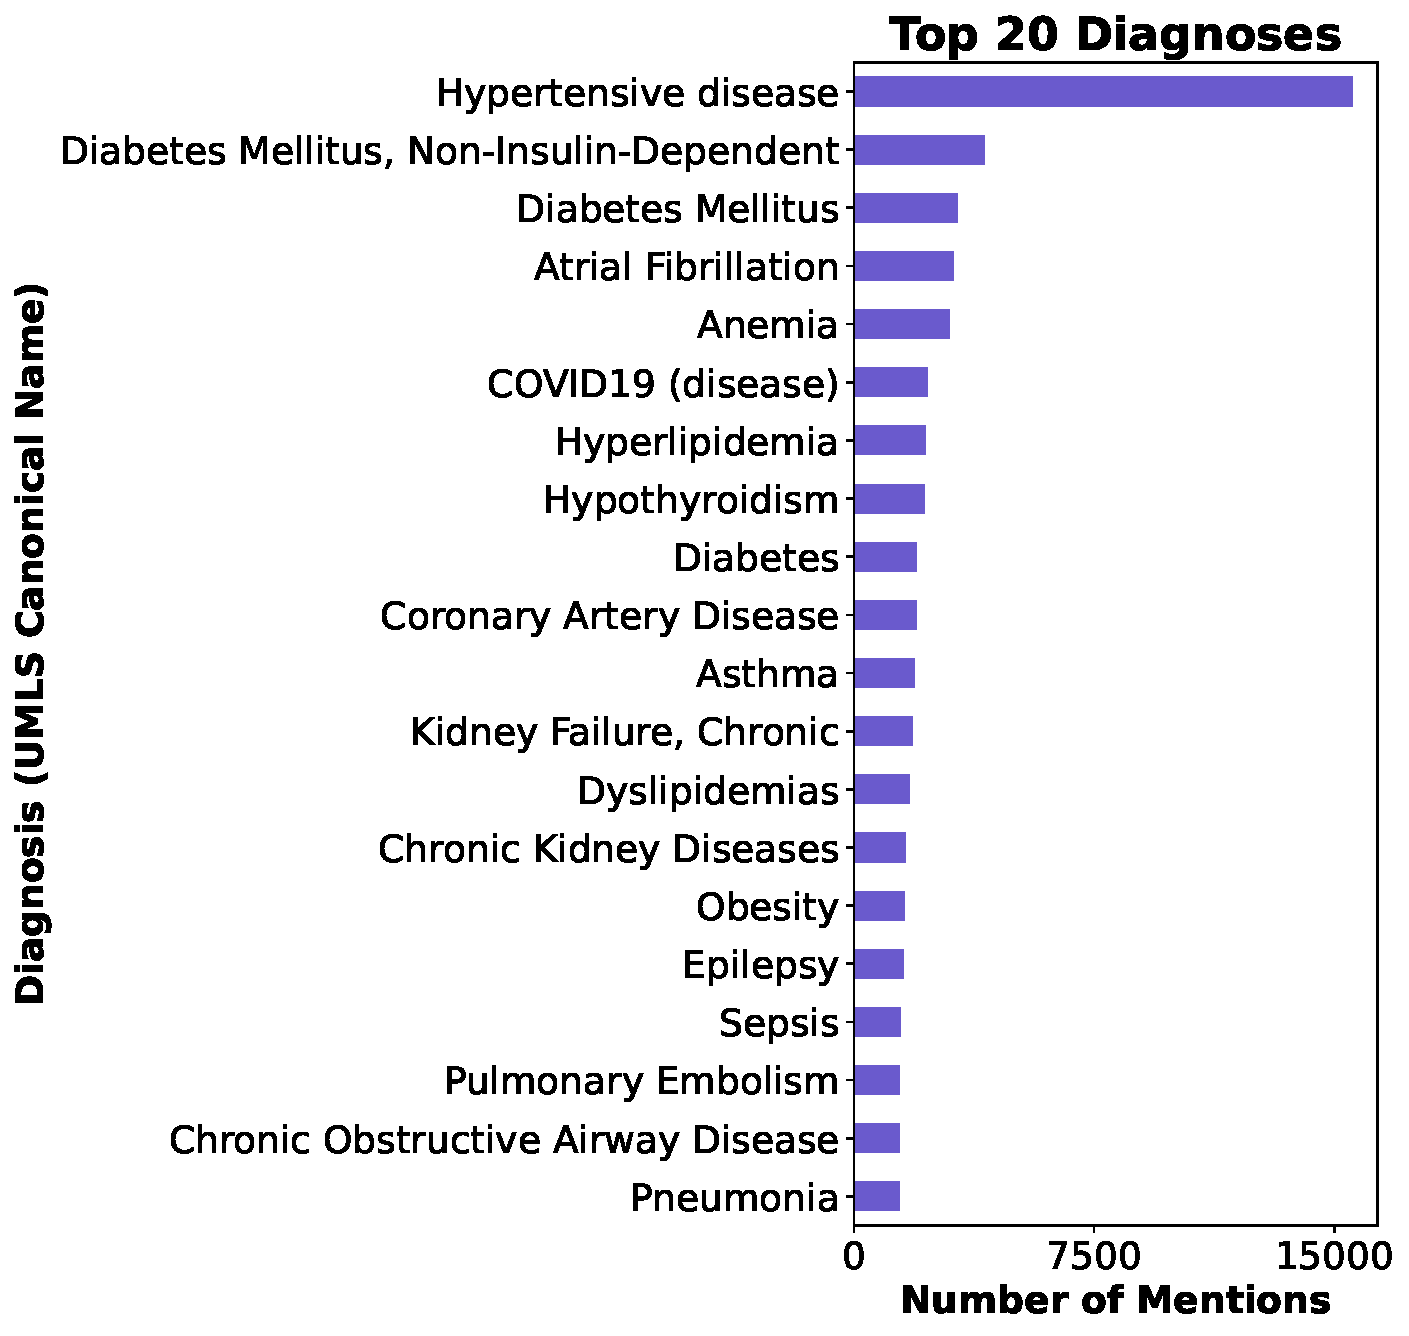
\includegraphics[width=0.99\linewidth]{Chapters/chapter-05/images/Scientific_data/Plots_tables/top_diagnoses_umls_corrected_lexical_tiebreak_paper_ready.pdf}}
        
        \label{ch05:fig:top_diagnoses}
    \end{minipage}}
    \hfill
    \subfloat[{Diagnosis co-occurrence heatmap.}]{\begin{minipage}[t]{0.6\textwidth}
        \centering
        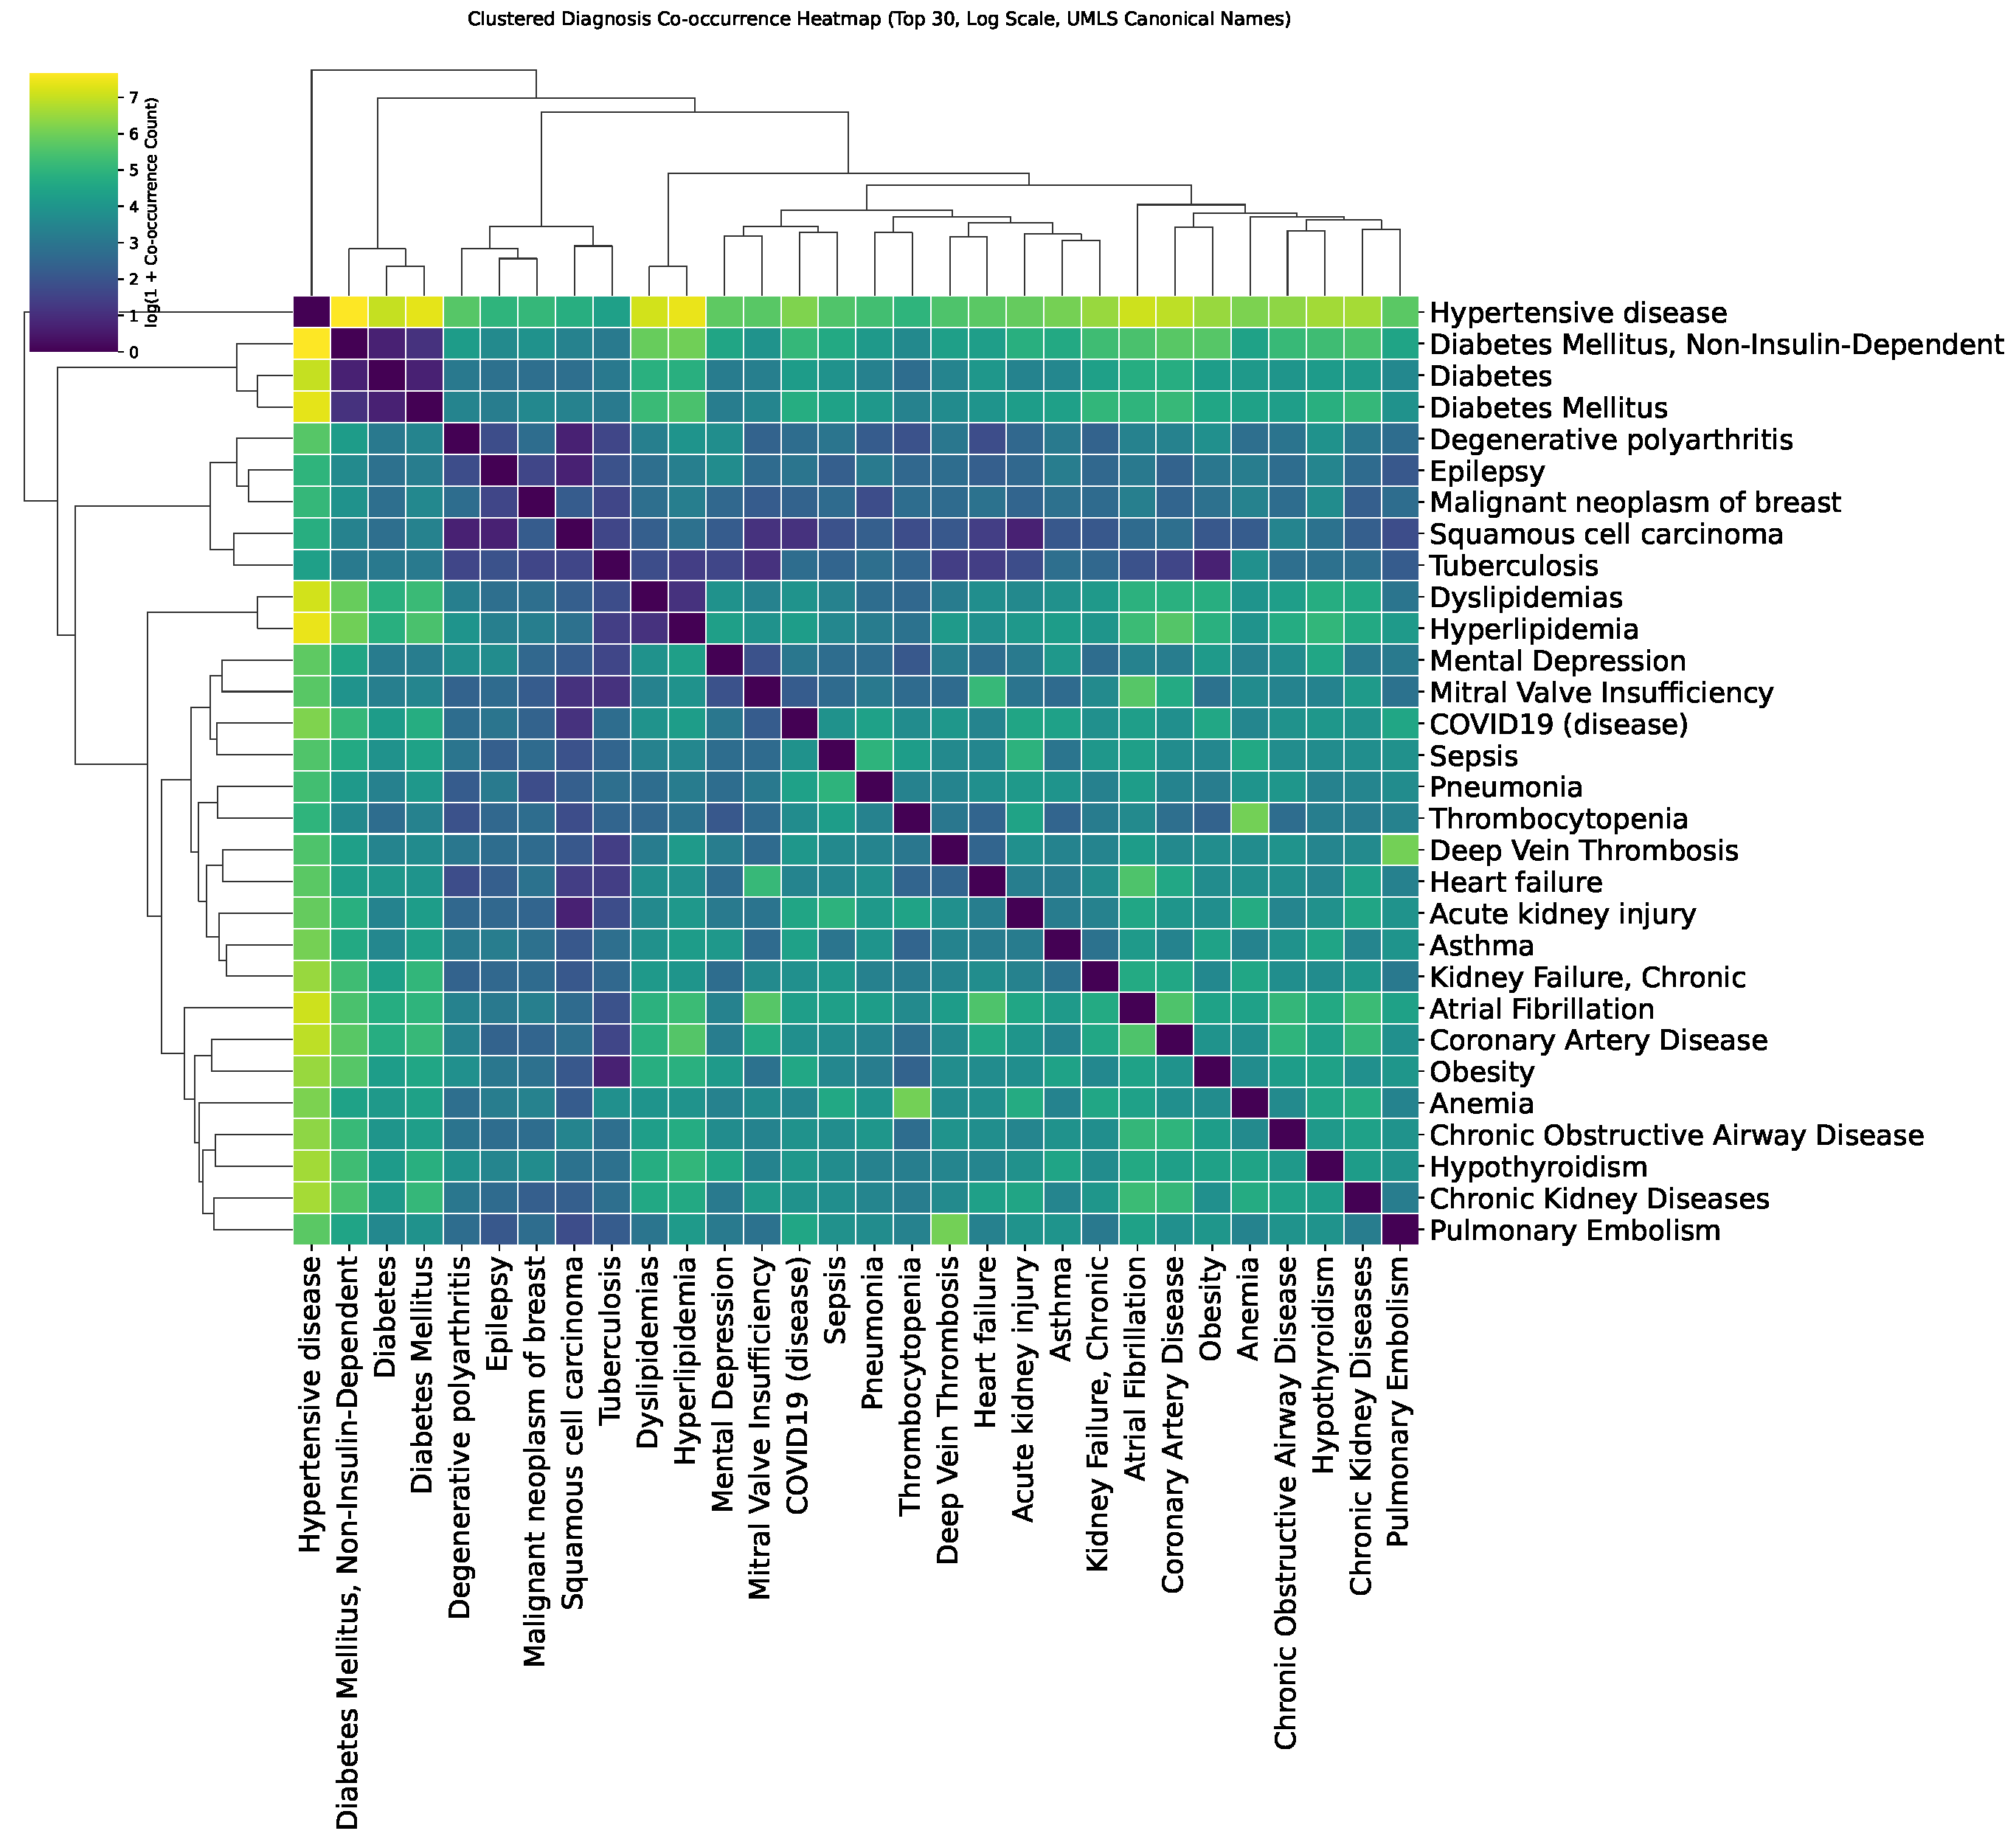
\includegraphics[width=0.99\linewidth]{Chapters/chapter-05/images/Scientific_data/Plots_tables/clustered_cooccurrence_heatmap_top30_corrected_lexical_tiebreak_canonical.pdf}
        
        \label{ch05:fig:diagnosis_cooccurrence}
    \end{minipage}}
    
    
    

\end{ChFiveFloatBody}
\caption{Frequency and co-occurrence patterns of UMLS-normalized diagnoses in PMOA-TTS. (a) The 20 most frequently mentioned diagnoses using canonical UMLS names. (b) Pairwise diagnosis co-occurrence (log-transformed counts) with hierarchical clustering, highlighting groups of frequently co-mentioned conditions.}\ChFiveFloatLabel{ch05:fig:diagnoses}
\end{figure}





